\subsection{Code analysis}

The code was analysed via the use of JadX, the program was able to decompile the code and present it in a readable manner. 
Many parts of the code, for instance classes, were obfuscated via the use of hashes.
Some of the functions and classes were readable and gave some clue of what they could represent. 
Via this method, a local database function was found which saves the users settings as shown in figure \ref{tim-database}.

\begin{figure}[H]
    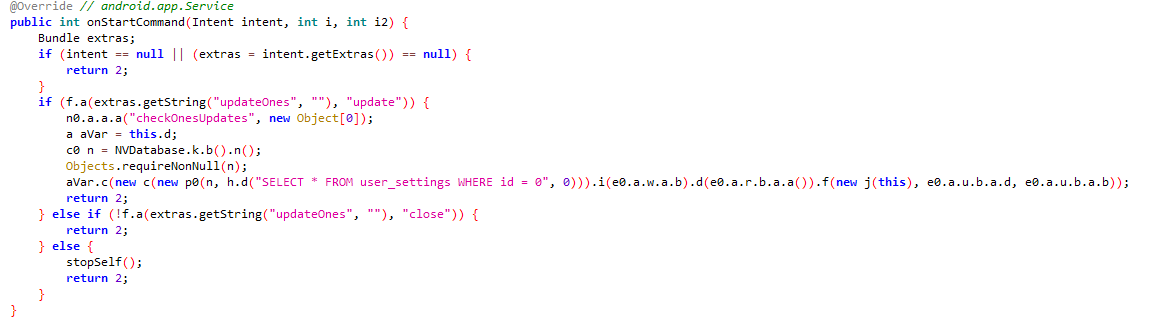
\includegraphics[width=1\textwidth]{codedatabase.PNG}
    \caption{Database hidden in the code}
    \label{tim-database}
\end{figure}

The code had an interface detailing a music app on the play store, the app itself isn’t harmful but the name of the app was Turkish. 
The app on the play store was however not specifically Turkish. 
There were also multiple lines spread throughout the code written in Turkish. 
This is further proof that this app was created by a Turkish developer.

\begin{figure}[H]
    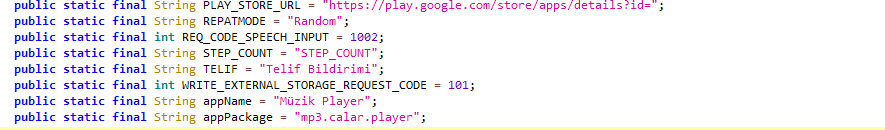
\includegraphics[width=1\textwidth]{musicplayer.PNG}
    \caption{musicplayer googleplay link}
    \label{tim-music}
\end{figure}

The application also had the option to enable and receive camera feed with the ability to hide it from the user. 
The code also was able to edit the user’s widgets, this was most likely how the app hid itself from the user. 
There was also code found that retrieved the users location.
 
The rest of the code was however hashed with no direct way to figure out what any of the code could mean. 
There were attempts to try and decrypt the code, but those did not turn out anything readable.

The program was marked as a banking Trojan, however it was not possible to find during the research related to this code.
It is still very likely that it is hidden in the hashed files but it was not decipherable, so that is just speculation.

